\documentclass{article}
\usepackage[backend=biber,citestyle=ieee]{biblatex}

\usepackage[english]{babel}
% \usepackage[swedish]{babel}

\usepackage{graphicx}
\usepackage{csquotes}
\usepackage{float}
\usepackage{datetime}
\usepackage[title]{appendix}


% \usepackage{a4wide} 

\usepackage{fancyhdr}   %page header
\pagestyle{fancy}

\usepackage{xcolor}
\usepackage{listings}

\definecolor{codegreen}{rgb}{0,0.6,0}
\definecolor{codegray}{rgb}{0.5,0.5,0.5}
\definecolor{codepurple}{rgb}{0.58,0,0.82}
\definecolor{backcolour}{rgb}{0.95,0.95,0.95}
\lstdefinestyle{mystyle}{
    backgroundcolor=\color{backcolour},   
    commentstyle=\color{codegreen},
    keywordstyle=\color{magenta},
    numberstyle=\tiny\color{codegray},
    stringstyle=\color{codepurple},
    basicstyle=\ttfamily\footnotesize,
    breakatwhitespace=false,         
    breaklines=true,                 
    captionpos=b,                    
    keepspaces=false,                 
    numbers=left,                    
    numbersep=5pt,                  
    showspaces=false,                
    showstringspaces=false,
    showtabs=false,                  
    tabsize=1
}
\lstset{style=mystyle}

\addbibresource{sources.bib}

\newcommand{\getauthor}{Oscar Fredriksson} %Author
\newcommand{\gettitle}{Visualization - Lab 2} %Title

\newdateformat{daymonthyear}{\ordinal{DAY} \monthname[\THEMONTH] \THEYEAR} %Date

\title{\gettitle}
\author{\getauthor}

\date{\daymonthyear\today} %Remove for swedish date

\begin{document}

    % Title 
    \pagenumbering{gobble}
    \maketitle
    \newpage

    % Page header and footer
    \pagenumbering{arabic}
    \fancyhf{}
    \lhead{\getauthor}
    \rhead{\gettitle}
    \rfoot \thepage

    \section{Visualization using Clip}
    The first part of the lab was to create a visualization using an IsoVolume and Clip filter. I could not find a vtk version of the IsoVolume filter I used in Paraview, so instead I used the contour filter to achieve a similar looking visualization. I started with the same values I used for lab 1, but I had to tweak the values for the clip filter slightly to achieve a similar visualization to what I got in lab 1. I found the filters along with syntax for how to use them by looking through the developer of vtks list of filters with examples \cite{vtk-examples}. An image of the visualization can be seen in figure \ref{fig:clip} and the written python code can be seen in appendix \ref{appendix:clip}.

    \begin{figure}[H]
        \centering
        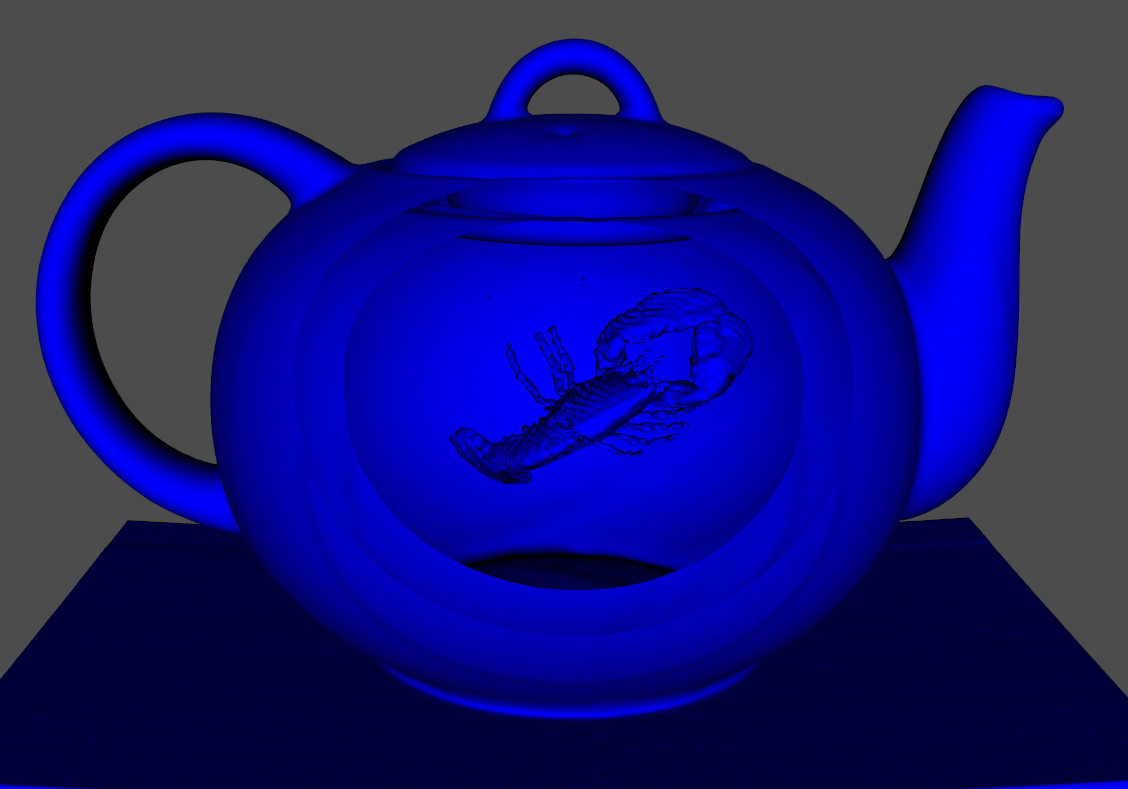
\includegraphics[width=0.75\textwidth]{../img/clip.png}
        \caption{A visualization of the teapot and lobster with a clip to see through the volume.}
        \label{fig:clip}
    \end{figure}

    % Document starts here
    \section{Visualization using Opacity}
    The second visualization uses two different contour values with different colours to highlight the lobster in yellow. I started with the same values I had in lab 1 for the two contours and the opacity, but had to lower the yellow contour slightly to make the visualization look similar to what was created in lab 1. The created visualization can be seen in figure \ref{fig:opacity} and the written python code can be seen in appendix \ref{appendix:opacity}.

    \begin{figure}[H]
        \centering
        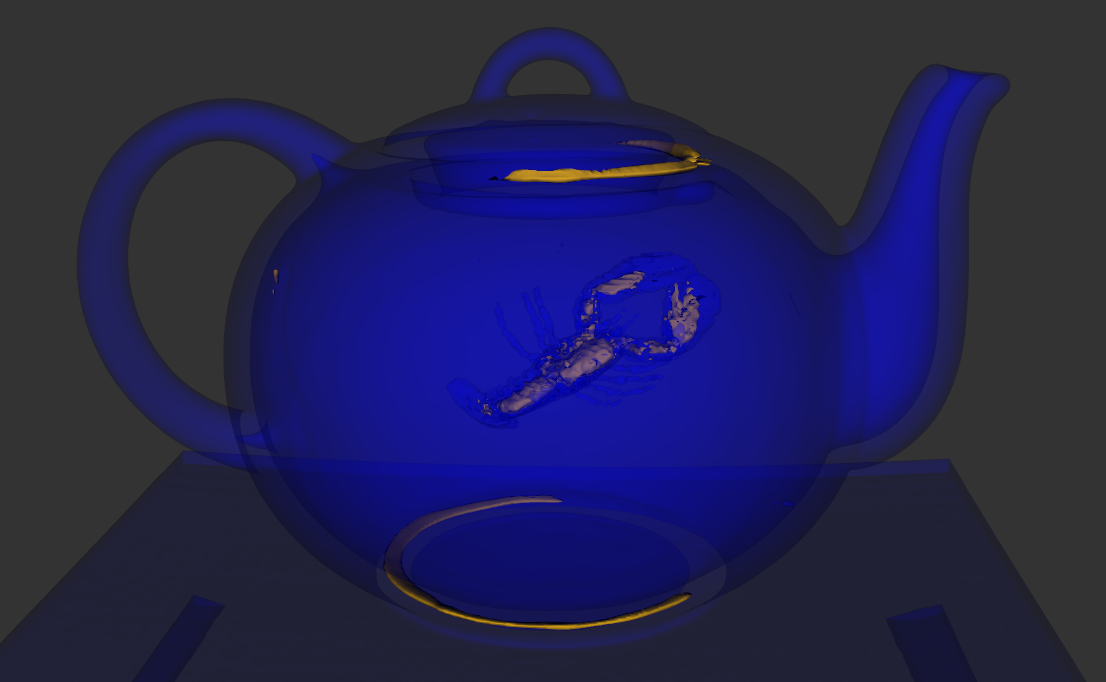
\includegraphics[width=0.75\textwidth]{../img/opacity.png}
        \caption{The  teapot  visualized  using  contour  with  values  30  (blue)  and  130(yellow) along with an opacity value of 0.2 to see the lobster inside.}
        \label{fig:opacity}
    \end{figure}

    \section{Conclusions}
    Two visualizations was created of the teapot that was near identicial to what was created using Paraview in lab 1. Figuring out how to use the different vtk filters was a bit challenging, especially since there wasn't much information to find online apart from the examples I found in \cite{vtk-examples}, so I had to rely on these to try and figure out how to use the filters. 

    After figuring out the syntax vtk worked very similarly to Paraview, and using the same parameters for the filters gave similar results, that after some tweaking could be considered near identical. The conclusions drawn from this lab is therefore that Paraview and vtk are two different tools that can be used to create similar visualizations.

    % Sources
    % \newpage
    % \printbibliography

    % Appendices
    \newpage
    \begin{appendices}

        \section{Clip visualization code}
        \label{appendix:clip}

        \lstinputlisting[language=python]{../src/clip.py}

        \newpage
        \section{Opacity visualization code}
        \label{appendix:opacity}

        \lstinputlisting[language=python]{../src/opacity.py}     

    \end{appendices}

\end{document}

% Centered figure with caption:
% \begin{figure}[H]
%     \centering
%     \includegraphics[width=1\textwidth]{%path} 
%     \caption{}
%     \label{fig:}
% \end{figure}

% Side by side figures:
% \begin{figure}[H]
%     \centering
%     \subfloat{{\includegraphics[width=0.46\textwidth]{%path} }}%
%     \qquad
%     \subfloat{{\includegraphics[width=0.46\textwidth]{%path} }}%
%     \caption{}
%     \label{fig:}
% \end{figure}

% Table with caption:
% \begin{table}[H]      
%     \begin{center}
%     \begin{tabular}{|c|c|} 
%         \hline
%         \textbf{} & \textbf{} \\\hline\hline
%          &  \\\hline 
%     \end{tabular}
%     \end{center}
%     \caption{}
%     \label{tab:}
% \end{table}